Die Interaktion mit Multi-Touch Eingaben wurde in einigen Veröffentlichungen thematisiert. Hierbei haben sich unterschiedliche Strategien, zur Kontrolle der Freiheitsgrade bei der Manipulation von dreidimensionalen Szenen, bewährt. (!?!?Des Weiteren wurden verschiedene Kriterien entwickelt, welche zur Bewertung von Multi-Touch Techniken dienen!?!?) Die im Rahmen dieser Arbeit entstandenen Ansätze, zur Umsetzung einer Multi-Touch basierten 3D Navigation, stützen sich auf diese Erkenntnisse.
\\\\
Dieses Kapitel stellt die in diesem Kontext wichtigsten verwandten Arbeiten vor. Hierzu beschreibt Abschnitt \ref{sec:related_sticky_tools} ein System zur 6DOF Interaktion mit Multi-Touch Tischen. In Abschnitt \ref{sec:related_balloon_selection} wird ein Ansatz zur Selektion von virtuellen Objekten, durch Touch Eingaben erläutert. Abschnitt \ref{sec:related_two_axis_valuator} erklärt die Umsetzung einer expliziten Geste zur Steuerung der 3D Rotation. Abschließend erfolgt in Abschnitt \ref{sec:diskussion_interaktion} eine Diskussion genannter Techniken.


\section{Sticky Tools}
\label{sec:related_sticky_tools}

Hancock et al. stellen ein System zur Steuerung von sechs Freiheitsgraden der dreidimensionalen Objekttransformation durch Multi-Touch Eingaben vor, welches sie Sticky Tools nennen \cite{hancock:2009}. Sie stützen sich dabei auf bekannte Techniken welche als \emph{force-based} bezeichnet werden. Hierbei soll das Gefühl erzeugt werden, die virtuelle Geometrie wie in der realen Welt durch direktes Anfassen zu manipulieren. 
\\\\
Die x- und y-Translation, uniforme Skalierung, sowie z-Rotation mit zwei Fingern hat sich im Alltag, durch den Umgang mit zweidimensionalen Touch-Anwendungen, bewährt. Es wird hierbei ein Initialkontakt mit der Geometrie bestimmt. Während der Bewegung der Finger, bleibt dieser durch Anwendung der genannten Transformationen, erhalten. Dieses \emph{Ankleben} der Objekte an die Berührungspunkte auf dem Bildschirm bezeichnen Hancock et al. als \emph{Sticky Fingers}-Technik \cite{hancock:2007,hancock:2009}.
\\\\
In dreidimensionalen Szenen wird die Translation um die z-Komponente erweitert. Hancock et al. nutzen für die Visualisierung der virtuellen Szene eine zweidimensionale Darstellung. Durch die perspektivische Verzerrung wächst der projizierte Abstand zweier Punkte auf einem Objekt, je mehr sich die Geometrie der Projektionsebene nähert. Sticky Tools simulieren den physikalischen Umgang mit nicht-elastischen Objekten. Aus diesem Grund wird auf eine Geste zur Skalierung verzichtet. Folglich wird die 2D Skalierungsgeste zur z-Translation eines Objekts genutzt.
\\\\
Neben der Rotation um die Hochachse ermöglicht die Manipulation in dreidimensionalen Szenen das Drehen von Objekten um Achsen auf der Bildfläche. Hancock et al. definieren letztere als \emph{flip}-Rotation. Um das Sticky Fingers Kriterium zu erhalten, wird diese Art der Rotation durch beidhändige Interaktion gesteuert. Hierbei werden durch das Aufsetzen zweier Finger einer Hand die direkten Kontaktpunkte auf der Geometrie festgelegt. Diese spannen einen Richtungsvektor auf, welcher die Rotationsachse definiert. Die Bewegung eines aufgesetzten Fingers der zweiten Hand im rechten Winkel zur Rotationsachse, legt den Grad der Flip-Rotation, sowie die Richtung der Drehung fest (siehe Abbildung \ref{fig:opposable_thumbs}).

\begin{figure}
	\begin{center}
		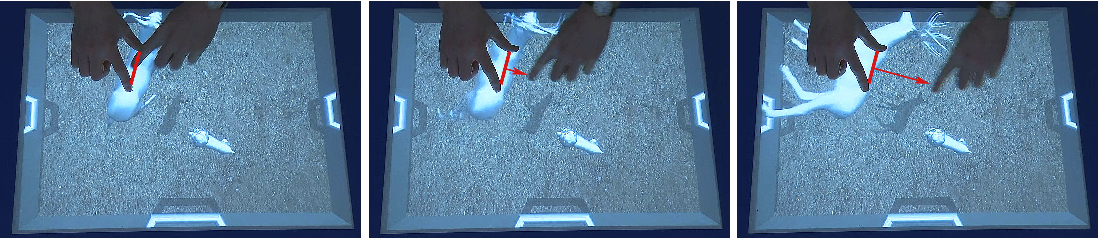
\includegraphics[width=12cm]{img/opposable_thumbs.pdf}
	\end{center}
	\caption{Durchführung der Opposable Thumbs Rotation im von Hancock et al. entwickelten System Sticky Tools \cite{hancock:2009}. Screenshots sind dem zugehörigen Video entnommen und durch eigene Visualisierungen erweitert worden \cite{hancock:2009:vid}.}
	\label{fig:opposable_thumbs}
\end{figure}


\section{Balloon Selection}
\label{sec:related_balloon_selection}

\begin{figure}
	\begin{center}
		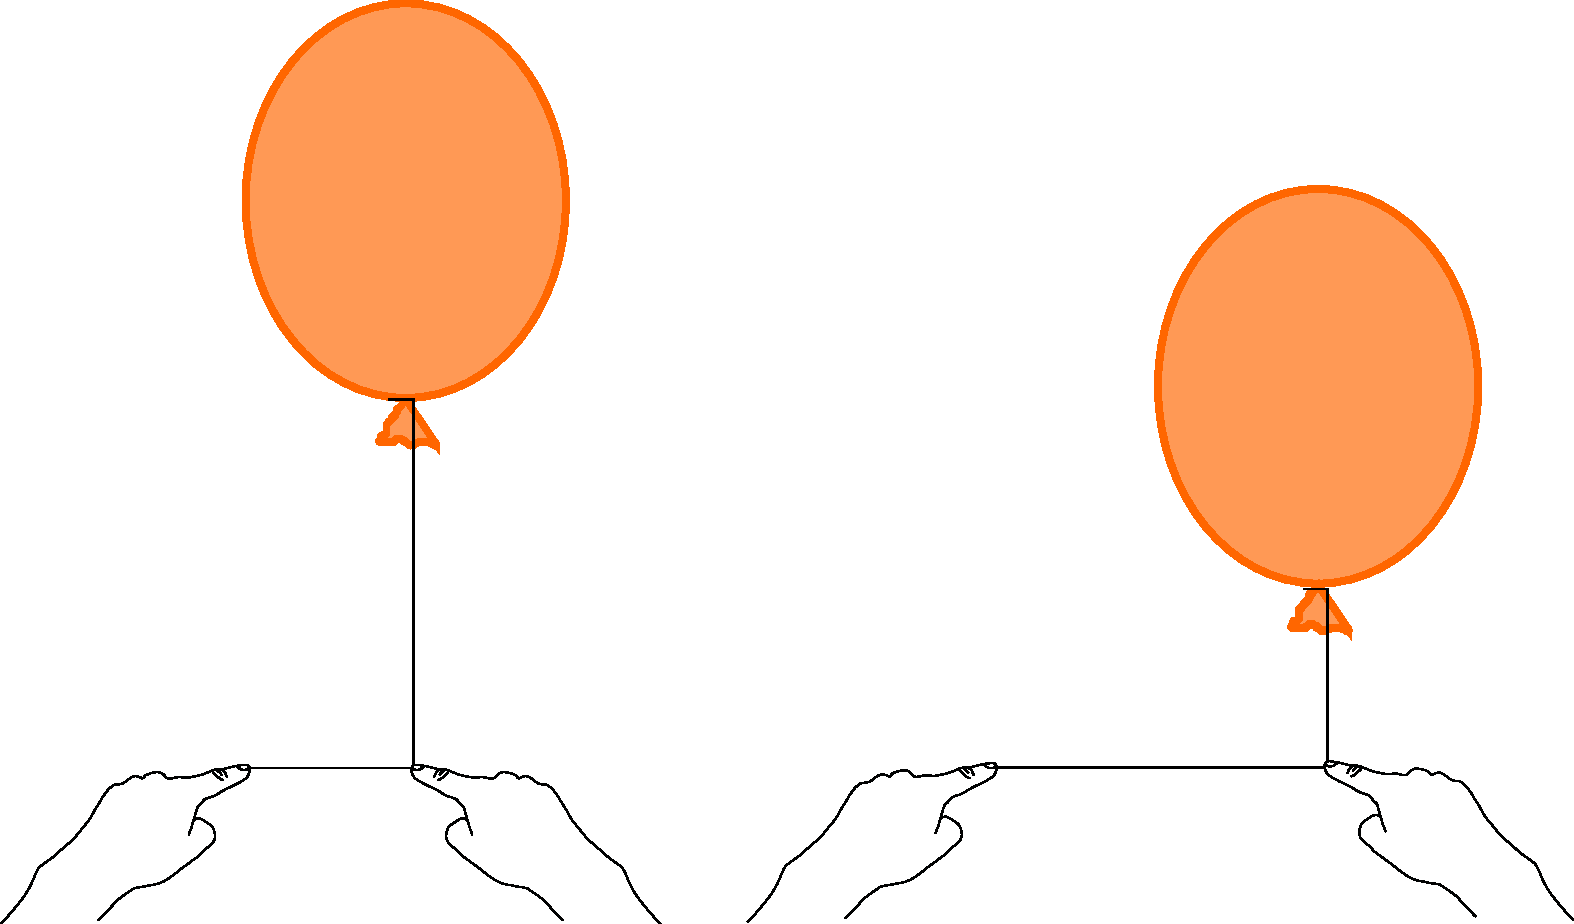
\includegraphics[width=8cm]{img/baloon_concept.pdf}
	\end{center}
	\caption{Aufstiegsveränderung eines mit Helium gefüllten Ballons.}
	\label{fig:baloon_concept}
\end{figure}

Balloon Selection ist eine von Benko und Feiner \cite{benko:2007} entwickelte Technik zur Multi-Touch basierten Selektion von virtuellen Objekten in dreidimensionalen Szenen. Dieser Ansatz ist inspiriert vom Umgang mit einem Helium Ballon. Demnach wird das Ende der Leine eines solchen Ballons mit einem Finger auf den Boden gehalten. Ein zweiter Finger fixiert die Leine an einem anderen Punkt auf dieser Ebene. Die Länge des fixierten Stückes bestimmt die Aufstiegsdistanz des Ballons. Folglich kann diese Distanz, sowie die Position des Ballons über dem Boden, durch das Verschieben der Handpositionen variiert werden. Abbildung \ref{fig:baloon_concept} visualisiert diese Metapher.
\\\\
Bei der Anwendung dieser Idee für die Selektion, wird eine Kugel als Selektionsobjekt genutzt. Die abgeleitete Geste wird durch das Aufsetzen zweier Finger in unmittelbarer Nähe zueinander initiiert. Hierbei dient der zuerst aufgelegte Finger als Ankerpunkt (nach Benko und Feiner \emph{anchor}). Der zweite Finger (nach Benko und Feiner \emph{stretching finger}) wird zur Festlegung der Leinenlänge verwendet. Hierzu bewegt der Nutzer seine Hand vom Ankerpunkt weg. Die Interaktionsleine wächst bis diese Bewegung sich in entgegen gesetzte Richtung umkehrt. Ab diesem Punkt ist die Länge der Leine fest und die Kugel steigt um die Länge der Distanzverkürzung zwischen den beiden Fingern orthogonal zur Tischebene nach oben. Der Ankerpunkt bestimmt durch Positionsveränderung die x- und y- Position des Ballons über der Interaktionsfläche.


\section{Two Axis Valuator}
\label{sec:related_two_axis_valuator}

Rousset et al. beschreiben eine Erweiterung von Scheurich und Stuerzlingers \emph{Two Axis Valuator} (im Folgenden TAV genannt) \cite{scheurich:2013,rousset:2014}. Der von Elisabeth Rousset et al. entwickelte TAV+ ist ein Modus zur einhändigen 3D Rotation durch die Verwendung von zwei Fingern. 
\\\\
Für die Bestimmung der Rotation entlang einer beliebigen Achse auf der Bildebene, wird die Bewegung der Zentrumsposition zwischen den aufgesetzten Fingern verfolgt. Die Rotation wird hierbei um die Achse, welche rechtwinklig zur Bewegungsrichtung steht und ebenfalls in der Bildebene liegt, durchgeführt. Als Rotationszentrum dient der Schwerpunkt des zu manipulierenden Objekts. Drehrichtung und Rotationsgrad werden von der Distanz und Richtung der Translation des Fingerzentrums abgeleitet. Zusätzlich kann die Rotation um die Achse zwischen Fingerzentrum und Rotationszentrum kontrolliert werden. Dies ist durch Orientierungsänderung des Vektors zwischen den Fingern möglich. Der verwendete Winkel, entspricht dem zwischen dem Vektor, vor der Bewegung und demselben danach. Abbildung \ref{fig:tav_plus} illustriert das Verfahren.

\begin{figure}
	\begin{center}
		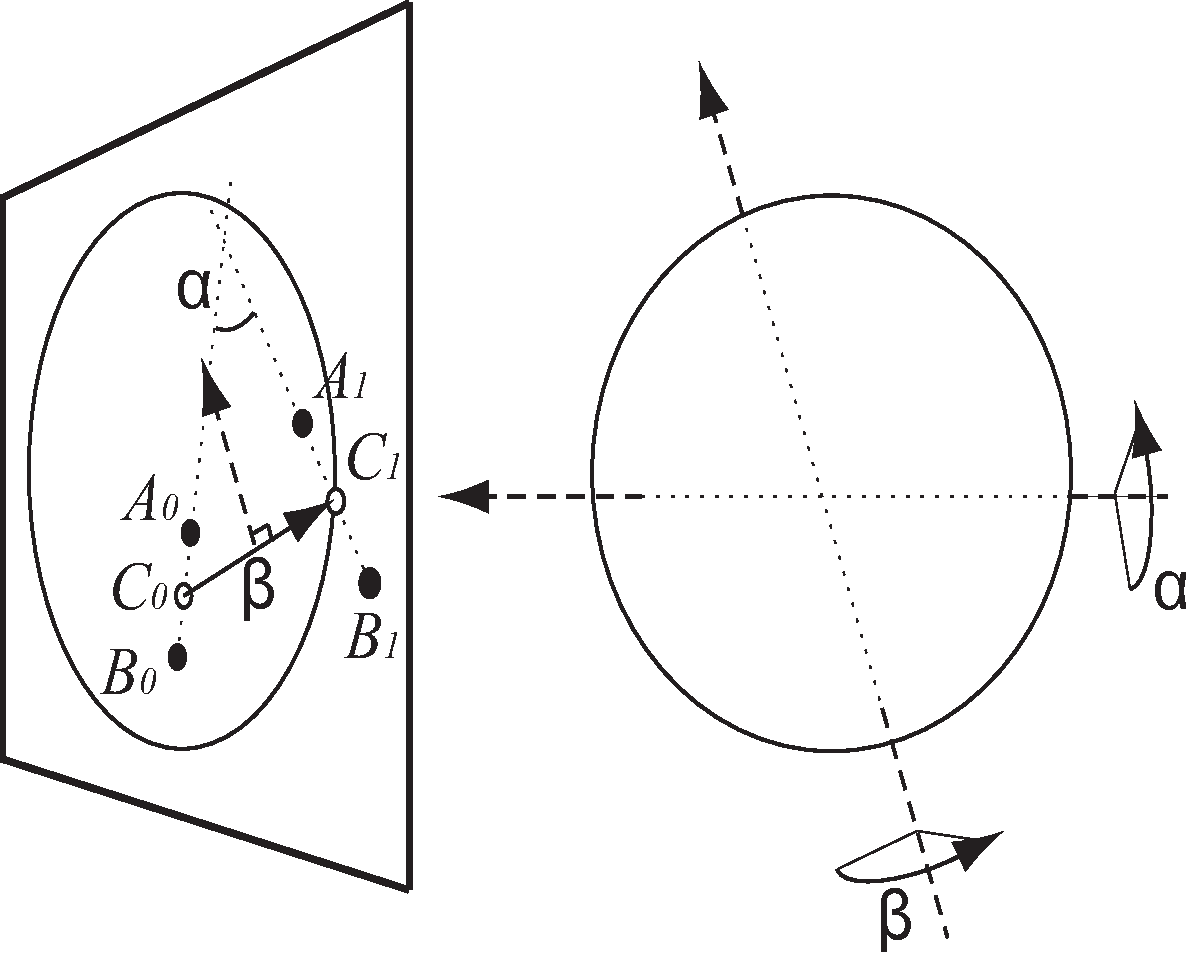
\includegraphics[width=10cm]{img/tav_plus.pdf}
	\end{center}
	\caption{Berechnung der dreidimensionalen Rotation TAV+ nach Rousset et al. \cite{rousset:2014}. Hierbei sind $A_i$ und $B_i$ die zwei zur Interaktion verwendeten Finger. $C_i$ ergibt sich als die Zenntrumsposition zwischen $A_i$ und $B_i$. $\alpha$ und $\beta$ sind die durch das Verfahren ermittelten Rotationswinkel. Diese Abbildung entstammt vollständig einer Veröffentlichung von Rousset et al \cite{rousset:2014}.}
	\label{fig:tav_plus}
\end{figure}


\section{Diskussion}
\label{sec:diskussion_interaktion}

Der direkte Umgang mit negativ-parallaxen Inhalten zeigt sich bei Touch-Interaktion mit stereoskopischen Visualisierungen als problematisch. Benko und Feiner kommen zu dem Schluss, dass Baloon Selection ein unter verschiedenen Umständen geeigneter Ansatz zur Selektion von über einer Interaktionsoberfläche liegenden virtuellen Objekten ist \cite{benko:2007}. Eine Umkehrung der Selektionsrichtung könnte das Verfahren auch für die 3D Multi-Touch Interaktion sinnvoll einsetzbar machen. Die Selektion von virtuellen Inhalten wird im Kontext dieser Arbeit nicht betrachtet. Jedoch ist eine explizite Höhenanpassung der Navigation, basierend auf den Erkenntnissen von Benko und Feiner, entstanden. Diese wird in Abschnitt \ref{sec:3d_translation} näher erläutert.
\\\\
Sticky Tools zeigen sich durch ihre physikalisch motivierte Entwicklung als intuitiv und nutzerfreundlich für die 3D Objektmanipulation.
\\\\
???CITE???
\\\\
Aus diesem Grund fließen einige der von Hancock et al. entwickelten Konzepte maßgeblich in die entstandene 3D Multi-Touch Navigation ein. Sticky Tools ersetzen die Funktionalität der herkömmlichen 2D Skalierungsgeste mit einer expliziten Höhenanpassung. Durch die perspektivische 2D Projektion geht hierbei visuell die direkte Verbindung zu den Kontaktpunkten auf der Geometrie nicht verloren. Stereoskopisches Rendering kann diese Illusion jedoch nicht gewährleisten. Zum Erhalt der Orthogonalität ist in diesem Anwendungsszenario eine uniforme Skalierung unabdingbar. 
\\\\
Der Umgang mit Objekten ist bei Sticky Tools auf geringe Entfernungen zur Bildebene begrenzt. Durch das Aufsetzen zweier Finger auf die Touch-Fläche werden Referenzpunkte auf der Geometrie festgelegt. Aus diesen Punkten wird eine Achse für die flip-Rotation abgeleitet. Weisen die Referenzpunkte einen Höhenunterschied auf, so wirkt sich dieser auf die hervorgerufene Drehung aus. Auf nahe Distanz zu manipulierenden Inhalten, ist die Höhendifferenz gut abschätzbar. Im Umgang mit komplexen Miniaturwelten und bei möglichen weiten Distanzen zu Objekten, wird diese Abschätzung zunehmend schwerer. Es ist in diesem Kontext von einer Beeinträchtigung der Nutzbarkeit der flip-Rotation auszugehen.
\\\\
TAV+ wird von Rousset et al. als 3D Rotationstechnik, welche für unerfahrene Nutzer einfach bedienbar ist, bewertet. Im direkten Vergleich mit anderen 3D Rotationstechniken schneidet TAV+ gut ab. Hierbei wird der Ansatz im Szenario einfacher Observationsaufgaben einzelner Objekte mit fester Position untersucht. Die Wahl des Rotationszentrums im Schwerpunkt der Geometrie erscheint in diesem Zusammenhang als sinnvoll. Bei der Navigation wird der Blickpunkt auf die Szene und somit alle virtuellen Objekte fortlaufend geändert. In diesem Fall wäre die Bedienung der TAV+ Rotation mit festem Rotationsreferenzpunkt sicherlich wenig nützlich. Abschnitt \ref{sec:3d_rotation} beschreibt wie der von Rousset et al. entwickelt abgeändert wurde, um einen effektive 3D Rotation der Navigation zu erreichen.
